%Set document format
\documentclass[11pt]{article}
\usepackage[margin=1in]{geometry}

%Set up packages
\usepackage{amsmath,amssymb,amsthm}
\usepackage{graphicx}
\usepackage{textcomp, gensymb}
\usepackage{float}
\usepackage{pdfpages}
\usepackage[hidelinks]{hyperref}
\usepackage{listings}
\usepackage{cancel}
\usepackage{subcaption}
\usepackage{caption}

\usepackage{mdframed}

\newcommand{\bm}{\boldsymbol}
\newcommand{\bI}{\mathbb{I}}
\newcommand{\bR}{\mathbb{R}}

\setlength\parindent{0pt}

\title{\bf Lab 3 \\ Supersonic Flow Over Diamond Airfoils}
\author{Andres's Contribution}
\date{}

\begin{document}
\maketitle


\noindent\makebox[\textwidth]{\rule{\textwidth}{0.2pt}}
\tableofcontents
\noindent\makebox[\textwidth]{\rule{\textwidth}{0.2pt}}
\pagebreak

\section{7.a} 
\begin{figure}[H]
    \centering
    \begin{subfigure}{0.475\linewidth}
        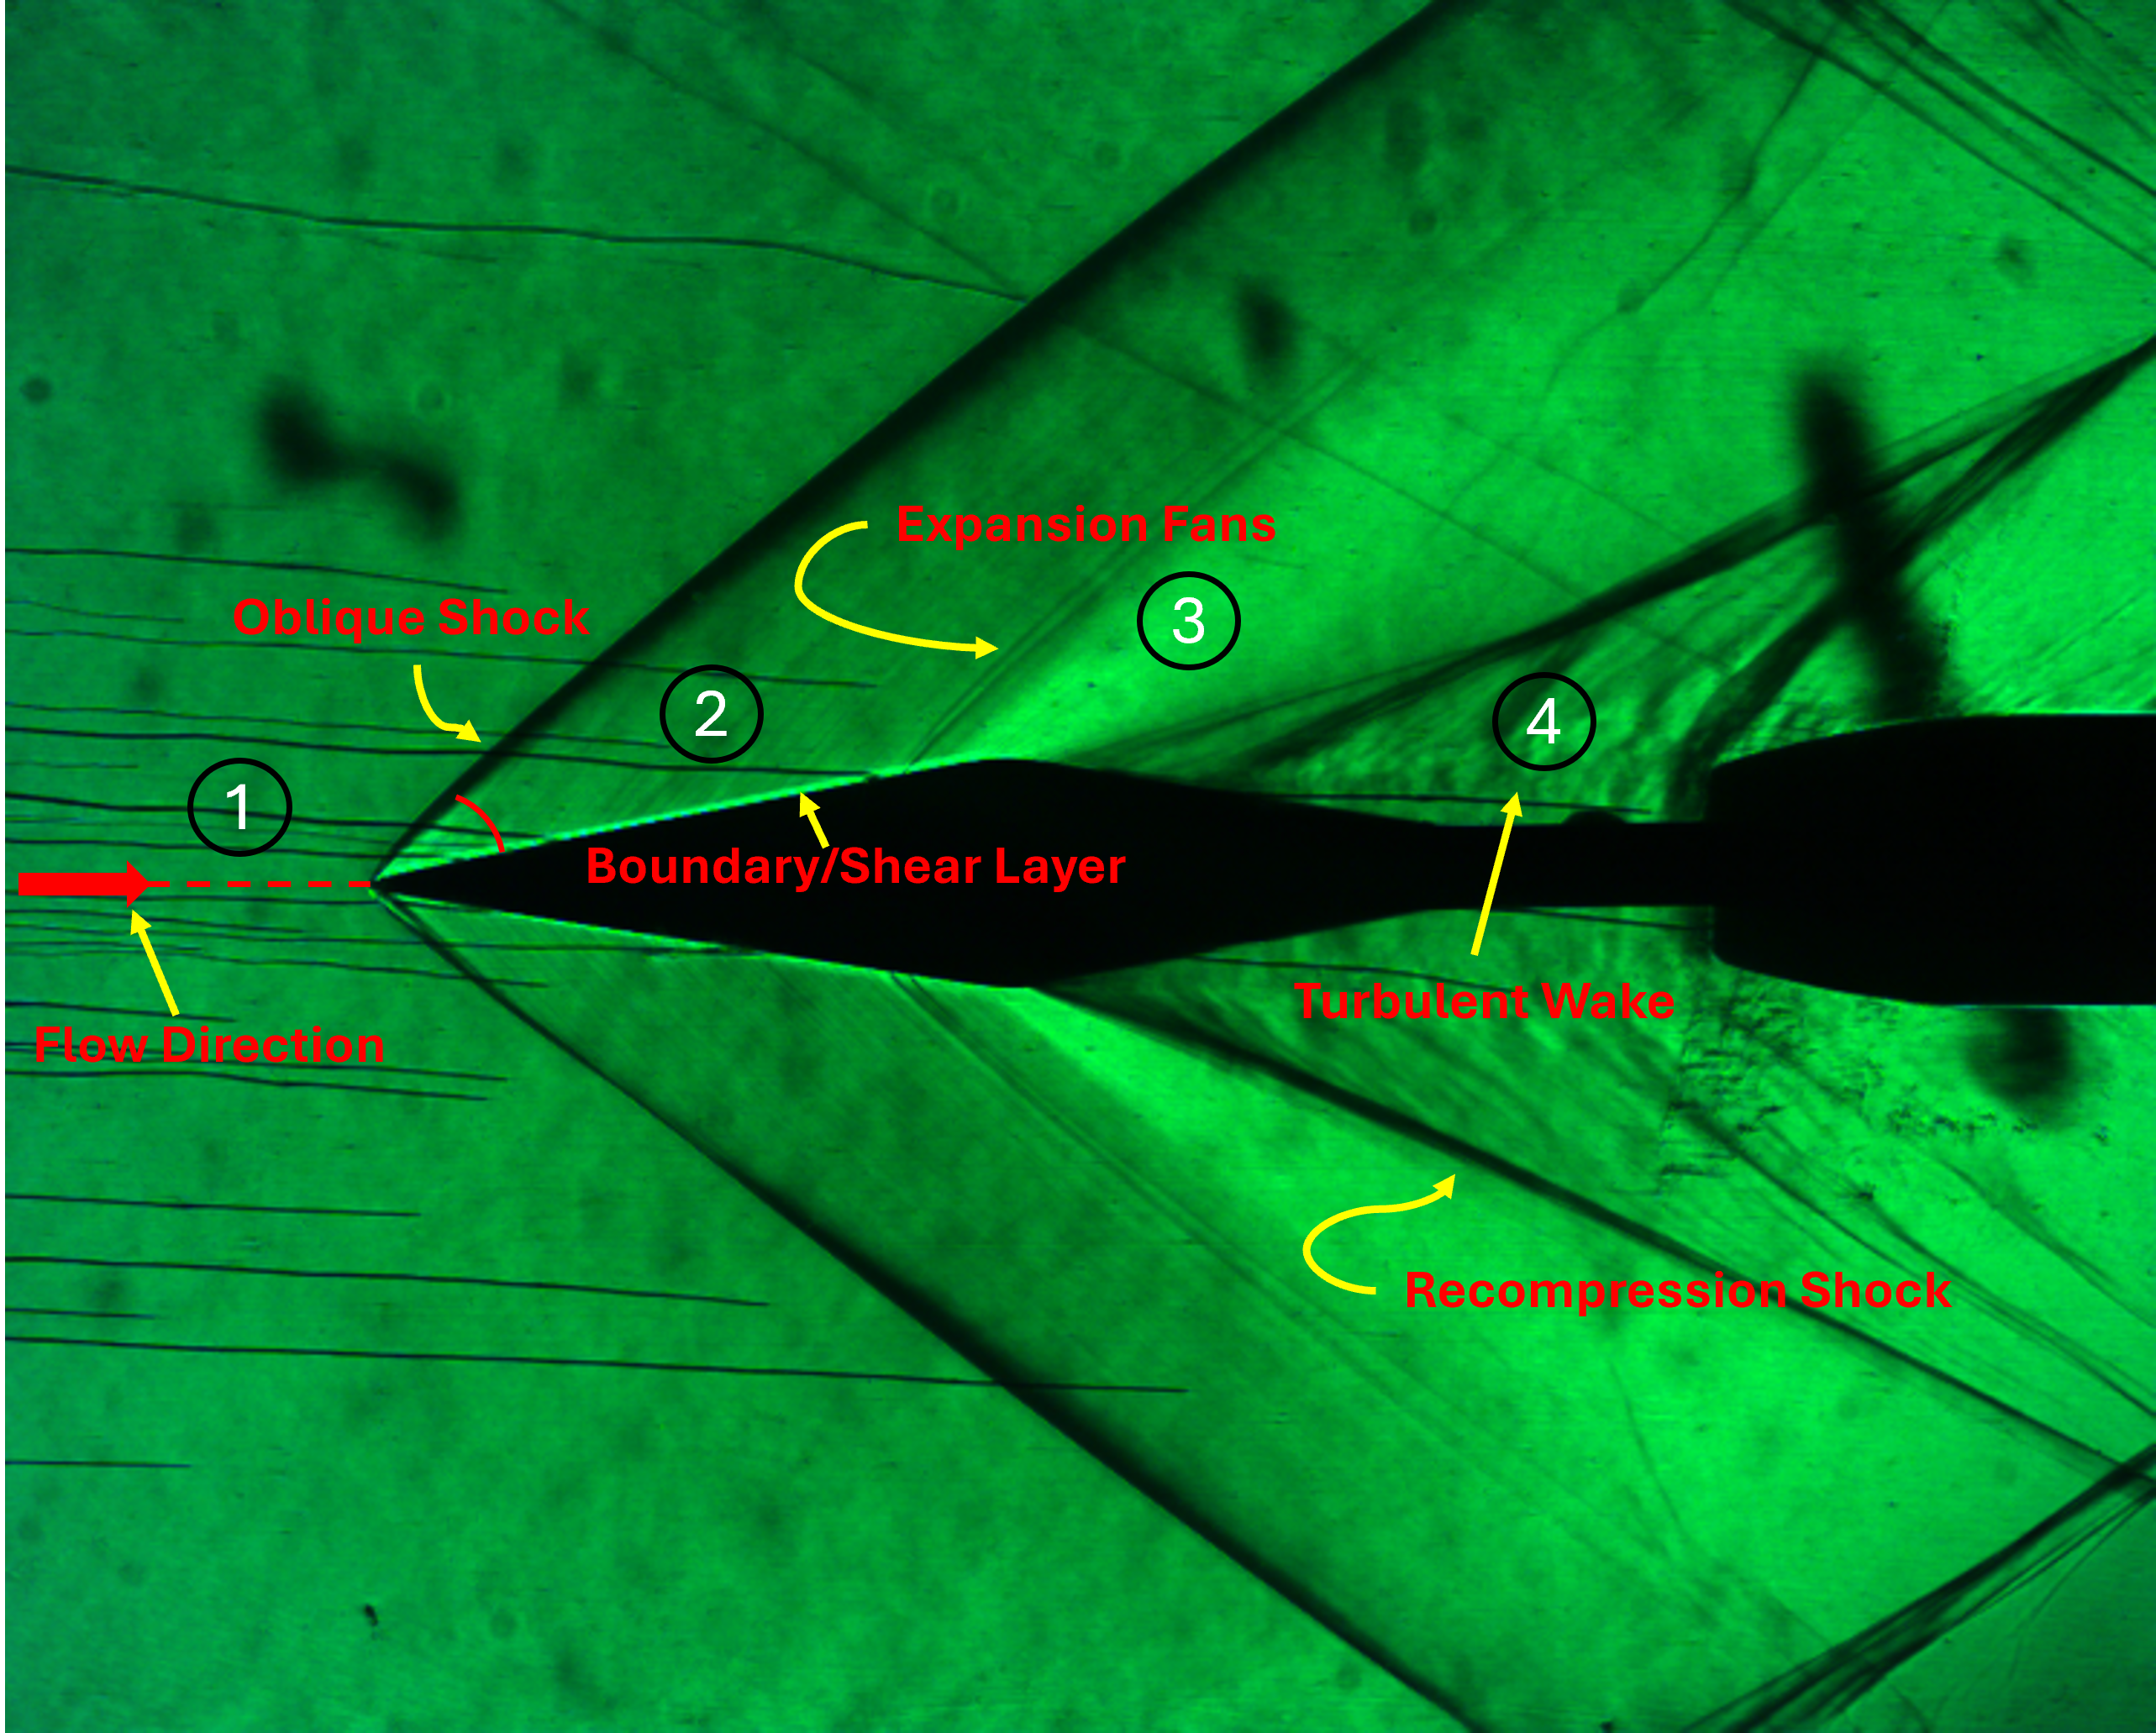
\includegraphics[width = \linewidth]{LabeledImages/Mach2_AoA0.png}
        \caption{Mach 2 flow at $0\degree$ angle of attack}
    \end{subfigure}
    \hspace{2.5mm}
    \begin{subfigure}{0.475\linewidth}
        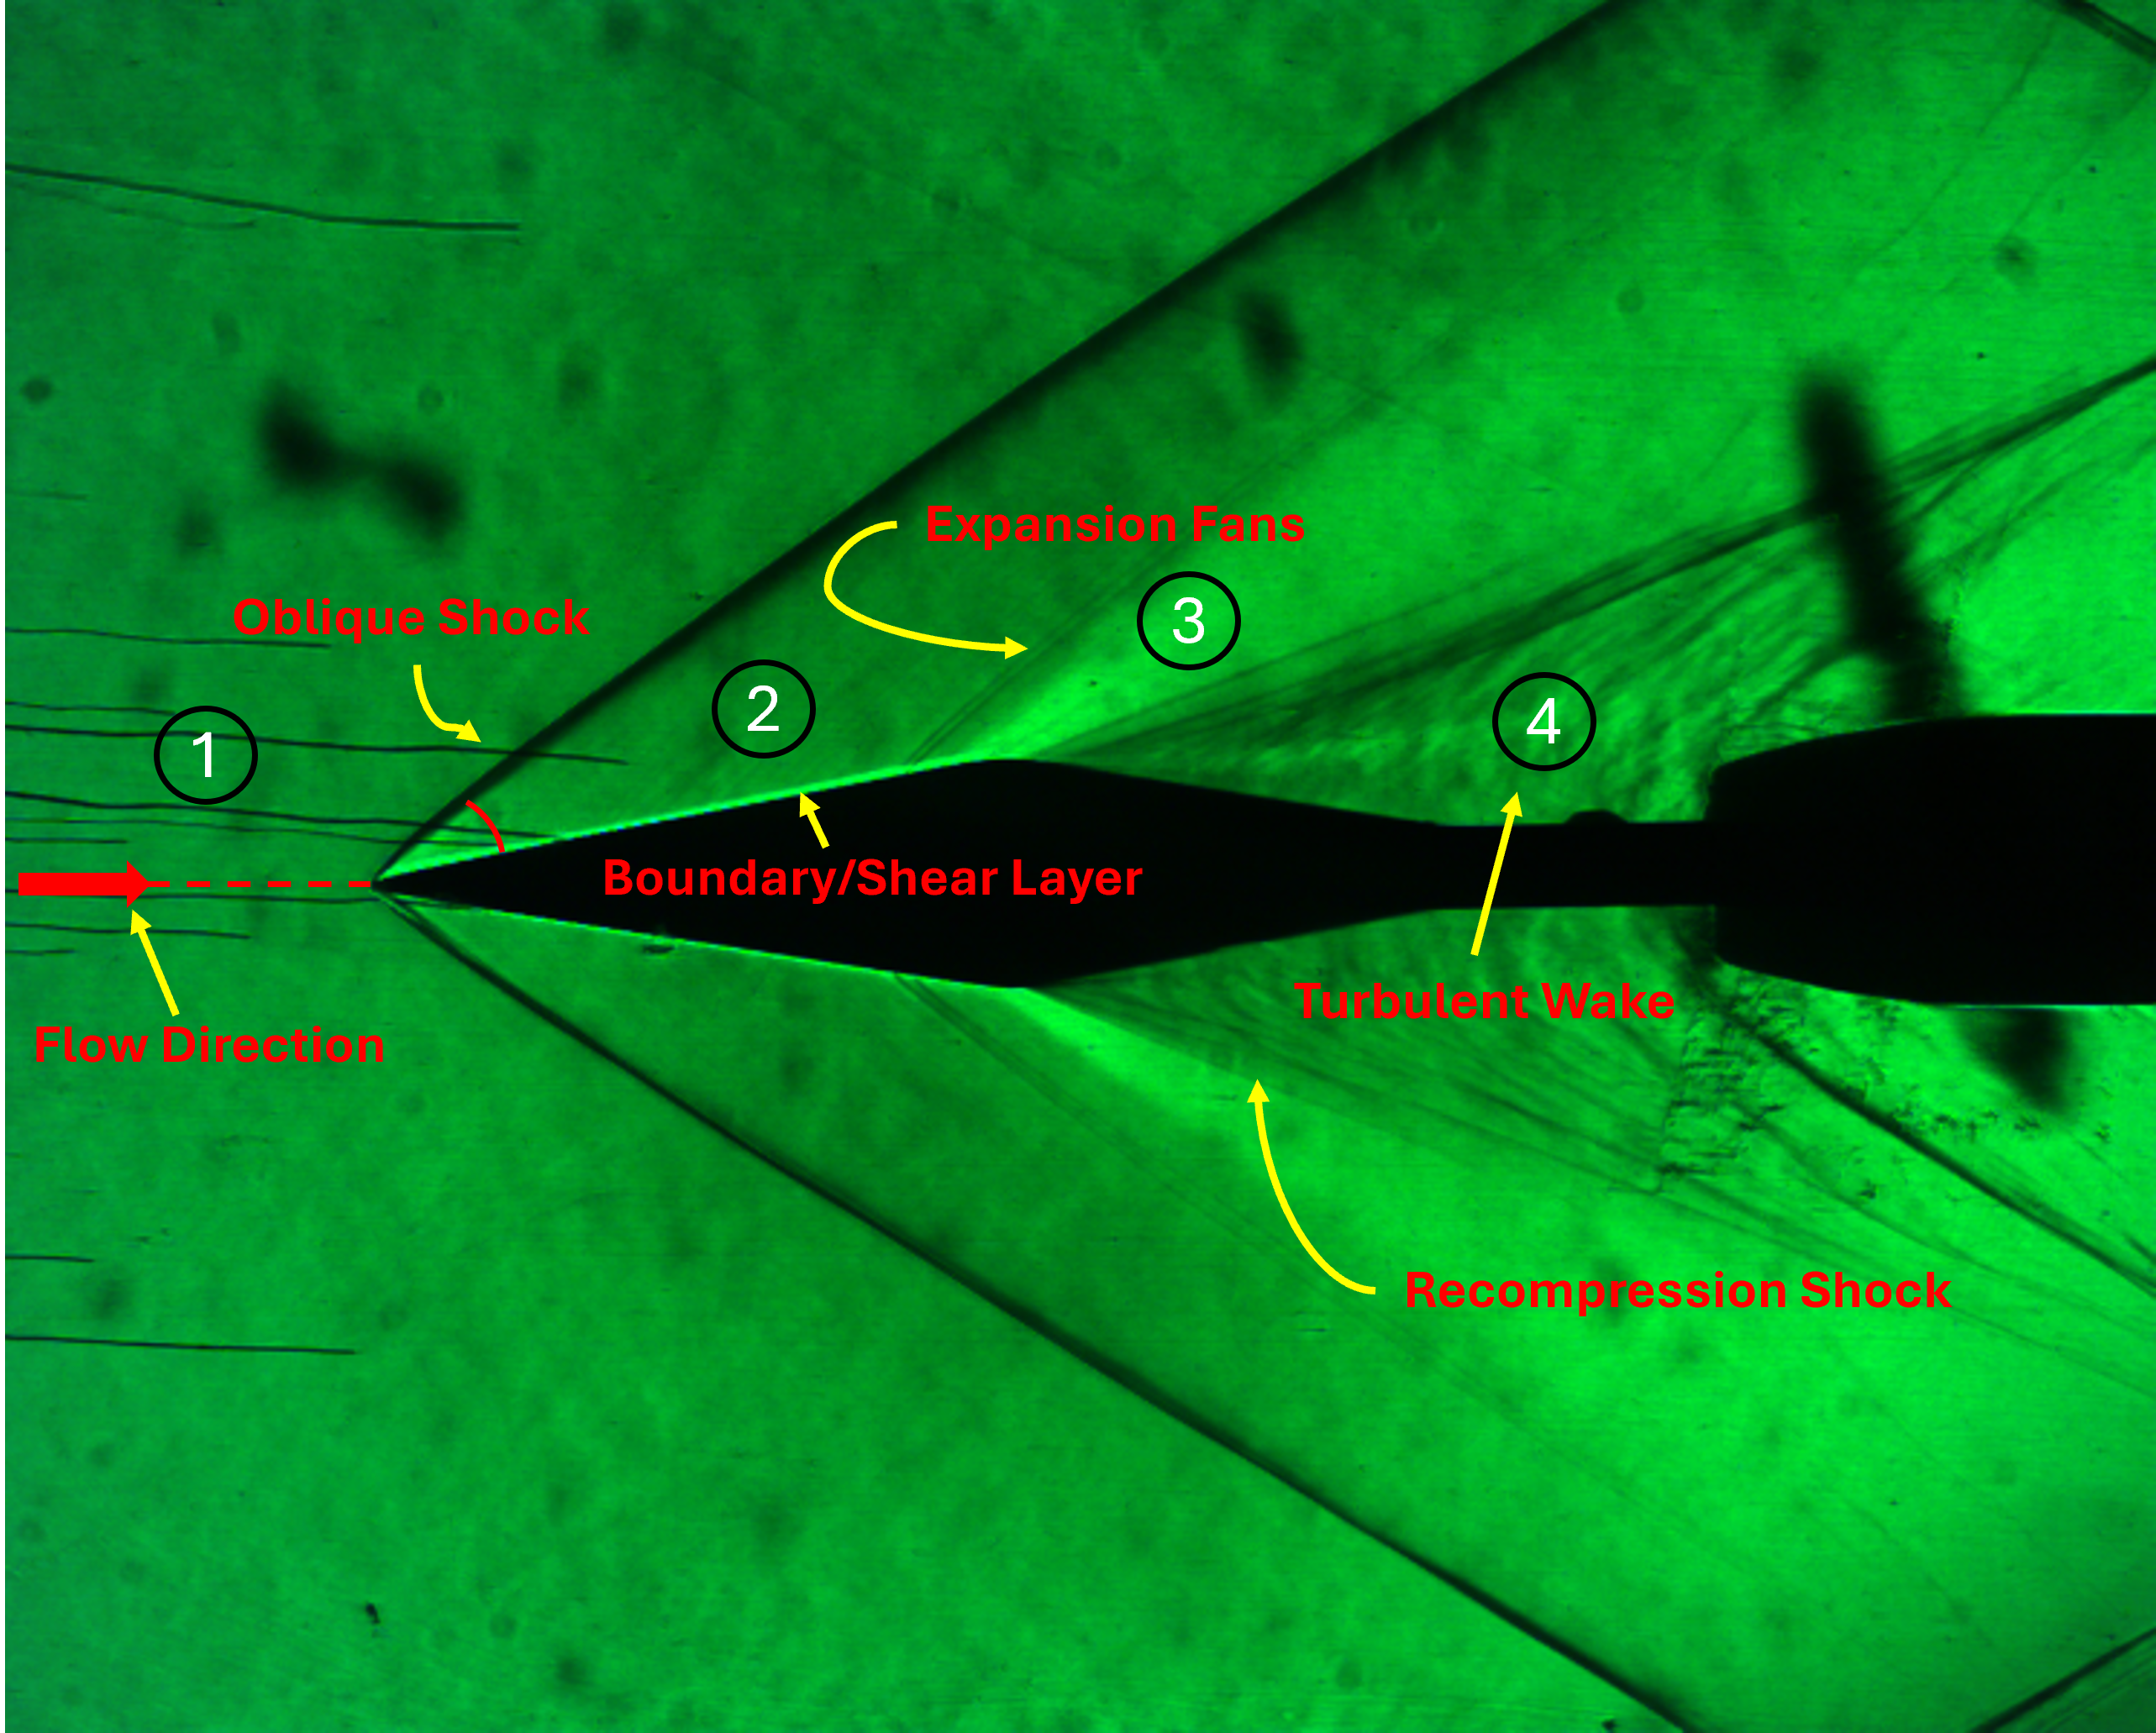
\includegraphics[width = \linewidth]{LabeledImages/Mach25_AoA0.png}
        \caption{Mach 2.5 flow at $0\degree$ angle of attack}
    \end{subfigure}
    \par\bigskip
    \begin{subfigure}{0.60\linewidth}
        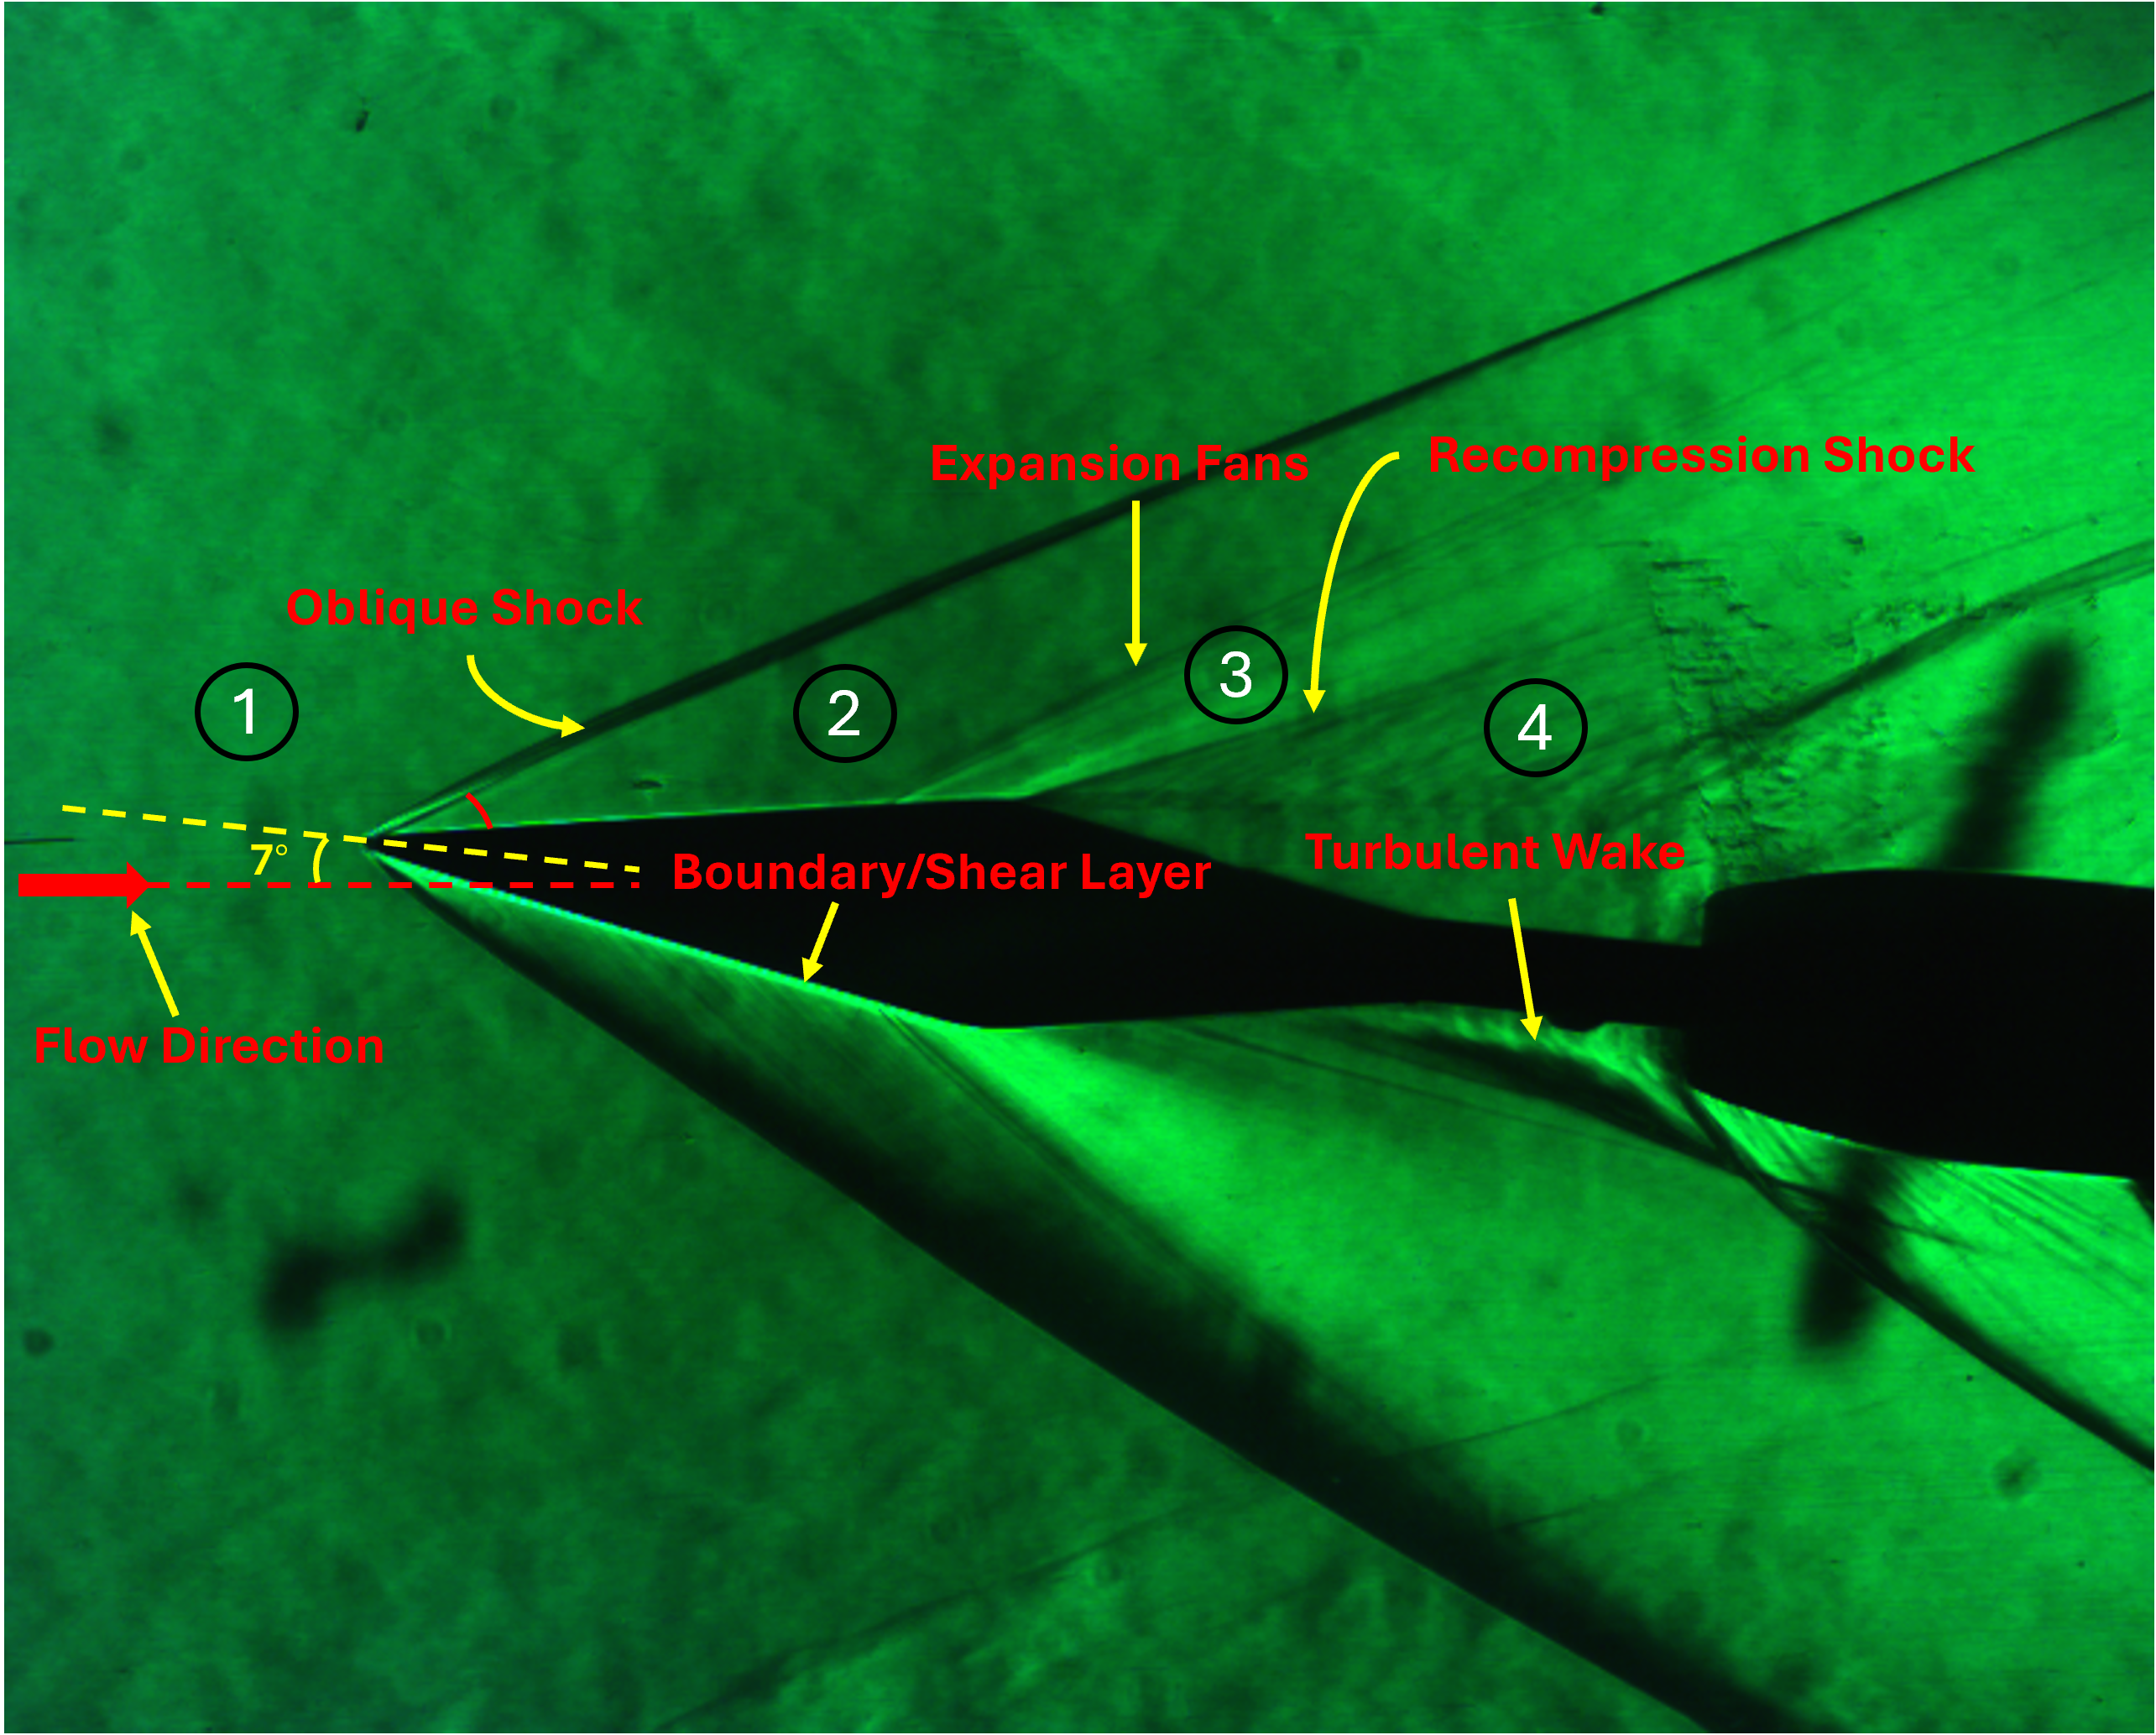
\includegraphics[width=\linewidth]{LabeledImages/Mach3_AoA7.png}
        \caption{Mach 3 flow at $7\degree$ angle of attack}
    \end{subfigure}
    \caption{Diamond Airfoil at different Machs and Angles of Attack}
    \label{images}
\end{figure}

Similarities and Differences between the different flows in Figure \ref{images} : 
\begin{itemize}
    \item Similarities:
    \begin{itemize}
        \item Each flow was visualized using a Vertical Schliern setup.
        \item The density gradients past the shocks and expansions is visibly clear. That is the density increase across the shock and density drop across the P-M fans are shown clearly by the light captured from the image.
        \item In each image there is a visible turbulent wake at the end of the diamond airfoil (zone 4).
        \item In each image, the expansion fans and recompression shocks seem to be occuring earlier than on a theoretical diamond airfoil. This discrepancy may be due to the test article not having sharp edges.
        \item Unlabeled : At the bottom of images (a) and (b) in Figure \ref{images}, a wave reflection can be seen as the shock interacts with the wall enclosing the test section.
    \end{itemize}
    \vspace{10mm}

    \item Differences:
    \begin{itemize}
        \item Between the Mach 2 and Mach 2.5 flows at $0\degree$ angle of attack, you can clearly see the shock angle becoming smaller. In addition, the expansion zone is smaller too.
        \item At Mach 3 and $7\degree$ angle of attack the boundary layer and expansion zone are much tighter on the top of the diamond (top in reference to image; originally the diamond airfoil was tilted $7\degree$ counterclockwise).
        \item The density gradient is much clearer and bigger on the bottom of the diamond airfoil at $7\degree$ angle of attack in Mach 3 flow. More of the flow is hitting that area.
    \end{itemize}
\end{itemize}

As Mach number increases, the shock wave angle decreases (refer to $\theta$-$\beta$-$M$ Relation). These images satisfy shock-expansion theory in this regard. However, as noted previously, the P-M expansion fans and recompression shocks occur much more upstream than shown on a theoretical diamond airfoil.

\subsection{Image Correction}
\begin{figure}[H]
    \centering
    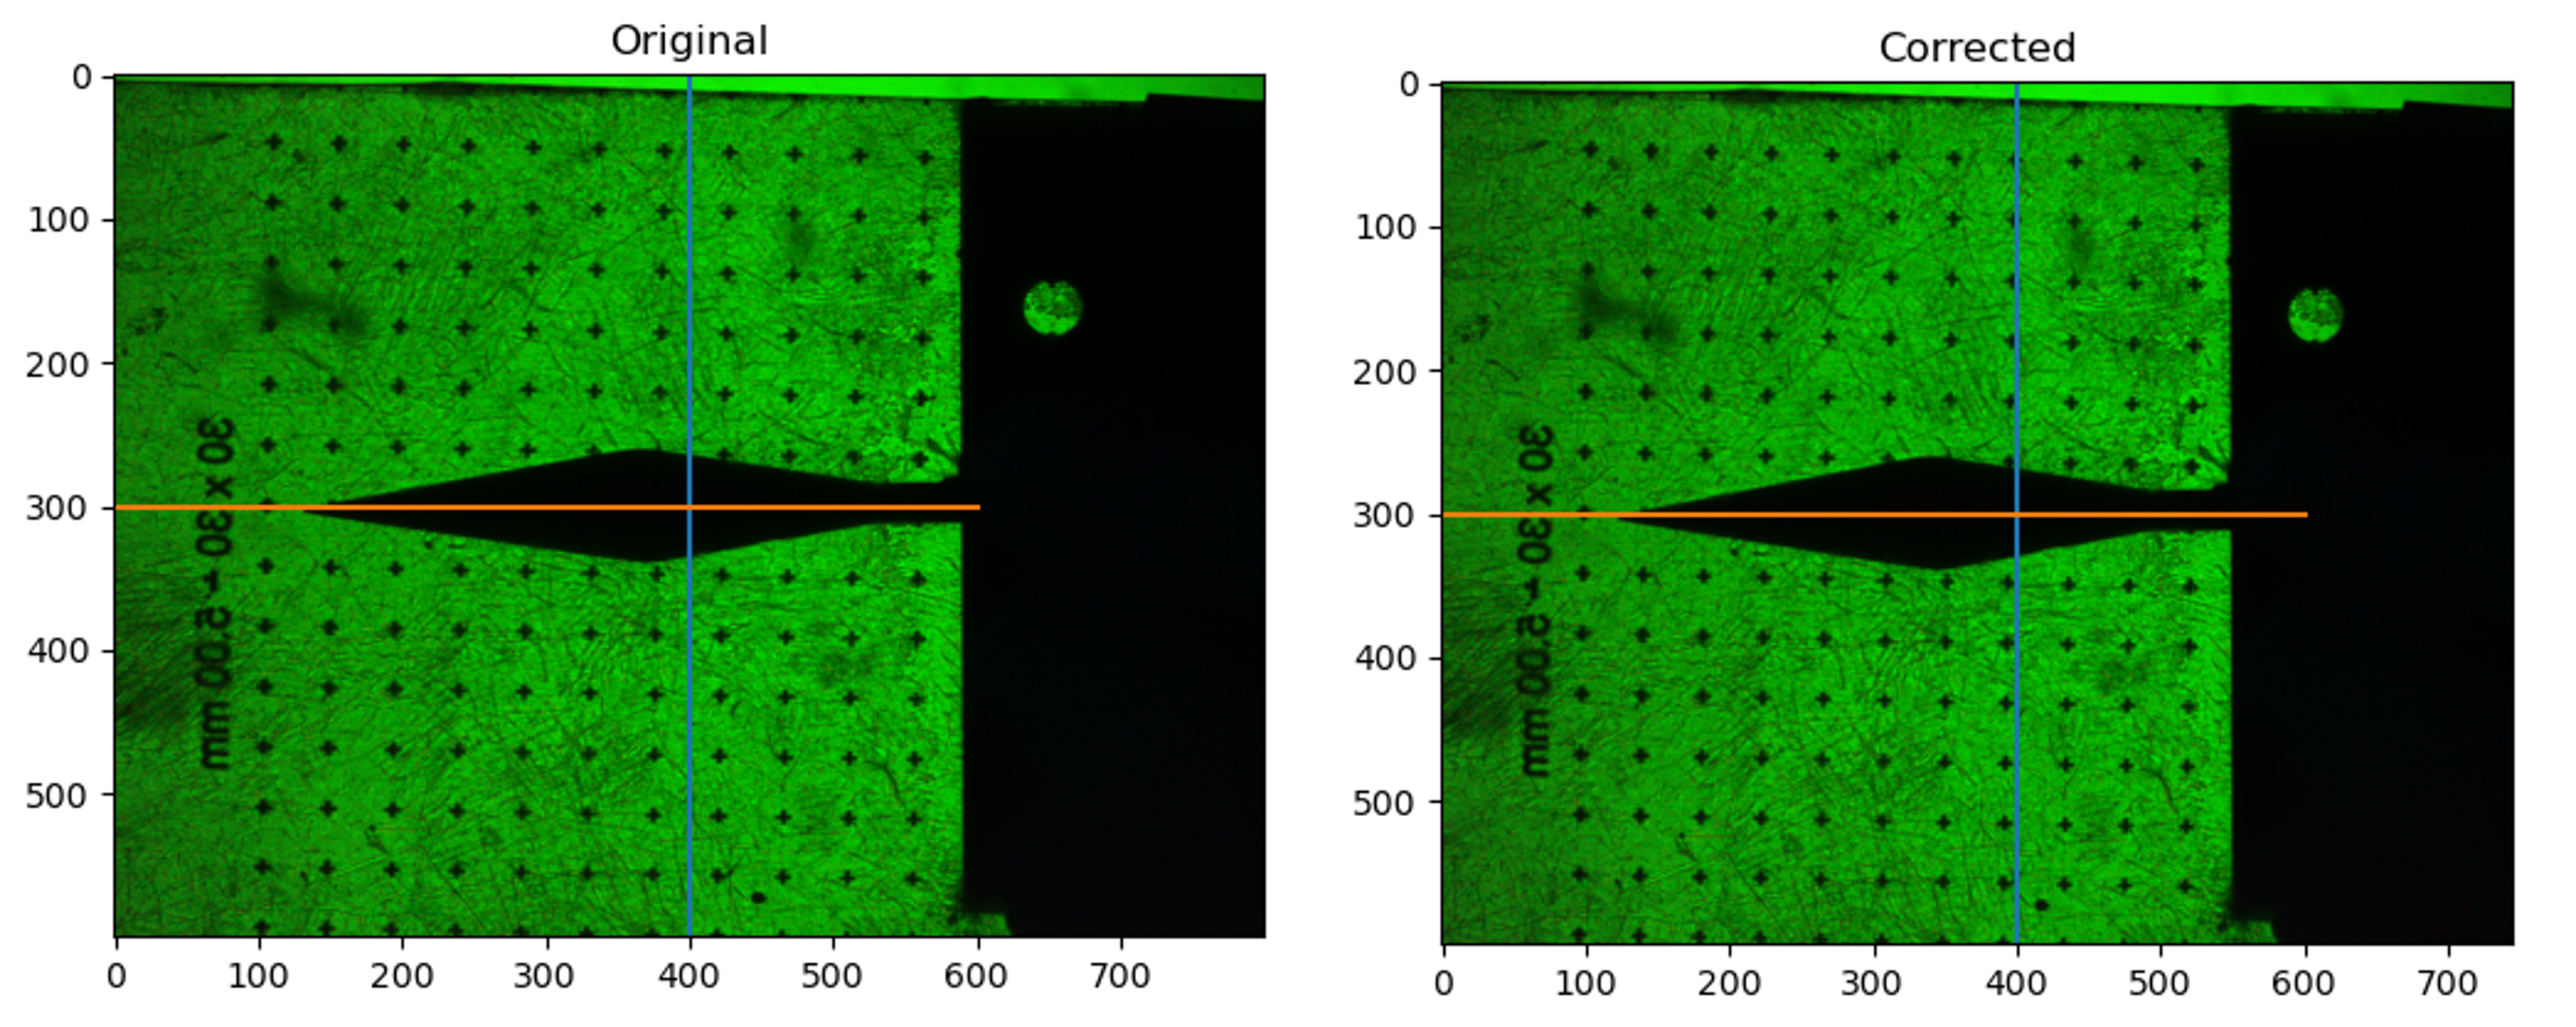
\includegraphics[width = \linewidth]{CorrectedImages/Diamond_GridImage_corrected_vs_raw.png}
    \caption{Corrected wind-off grid image, Raw vs Corrected}
    \label{correction}
\end{figure}

Given the grid image for correction, there was a noticable distortion as the images were corrected for a stretch along the horizontal. 
\vspace{5mm}

The raw resolution used was $800$ x $600$ pixels. After correction this became $745$ x $600$ pixels.
\vspace{2.5mm}

A calibration factor was calculated using this formula:
\begin{equation*}
    f = \dfrac{d_{\text{px}}}{n\cdot (5)}
\end{equation*}

The distance between each grid point is $5\, \text{mm}$ and $10$ grid points were used to measure the pixel distance along the grid making $n = 10$. It was found that $f_{x} = 9.06\, \text{pixel/mm}$ and $f_{y} = 8.44\, \text{pixel/mm}$. Thus there were more pixels in the horizontal direction for the same distance on the grid than in the vertical direction. Therefore the horizontal resolution was corrected by $800\cdot (f_{y}/f_{x}) \approx 745\, \text{px}$. This makes the aspect ratio now approximatly $1:1$.


\begin{figure}[H]
    \centering
    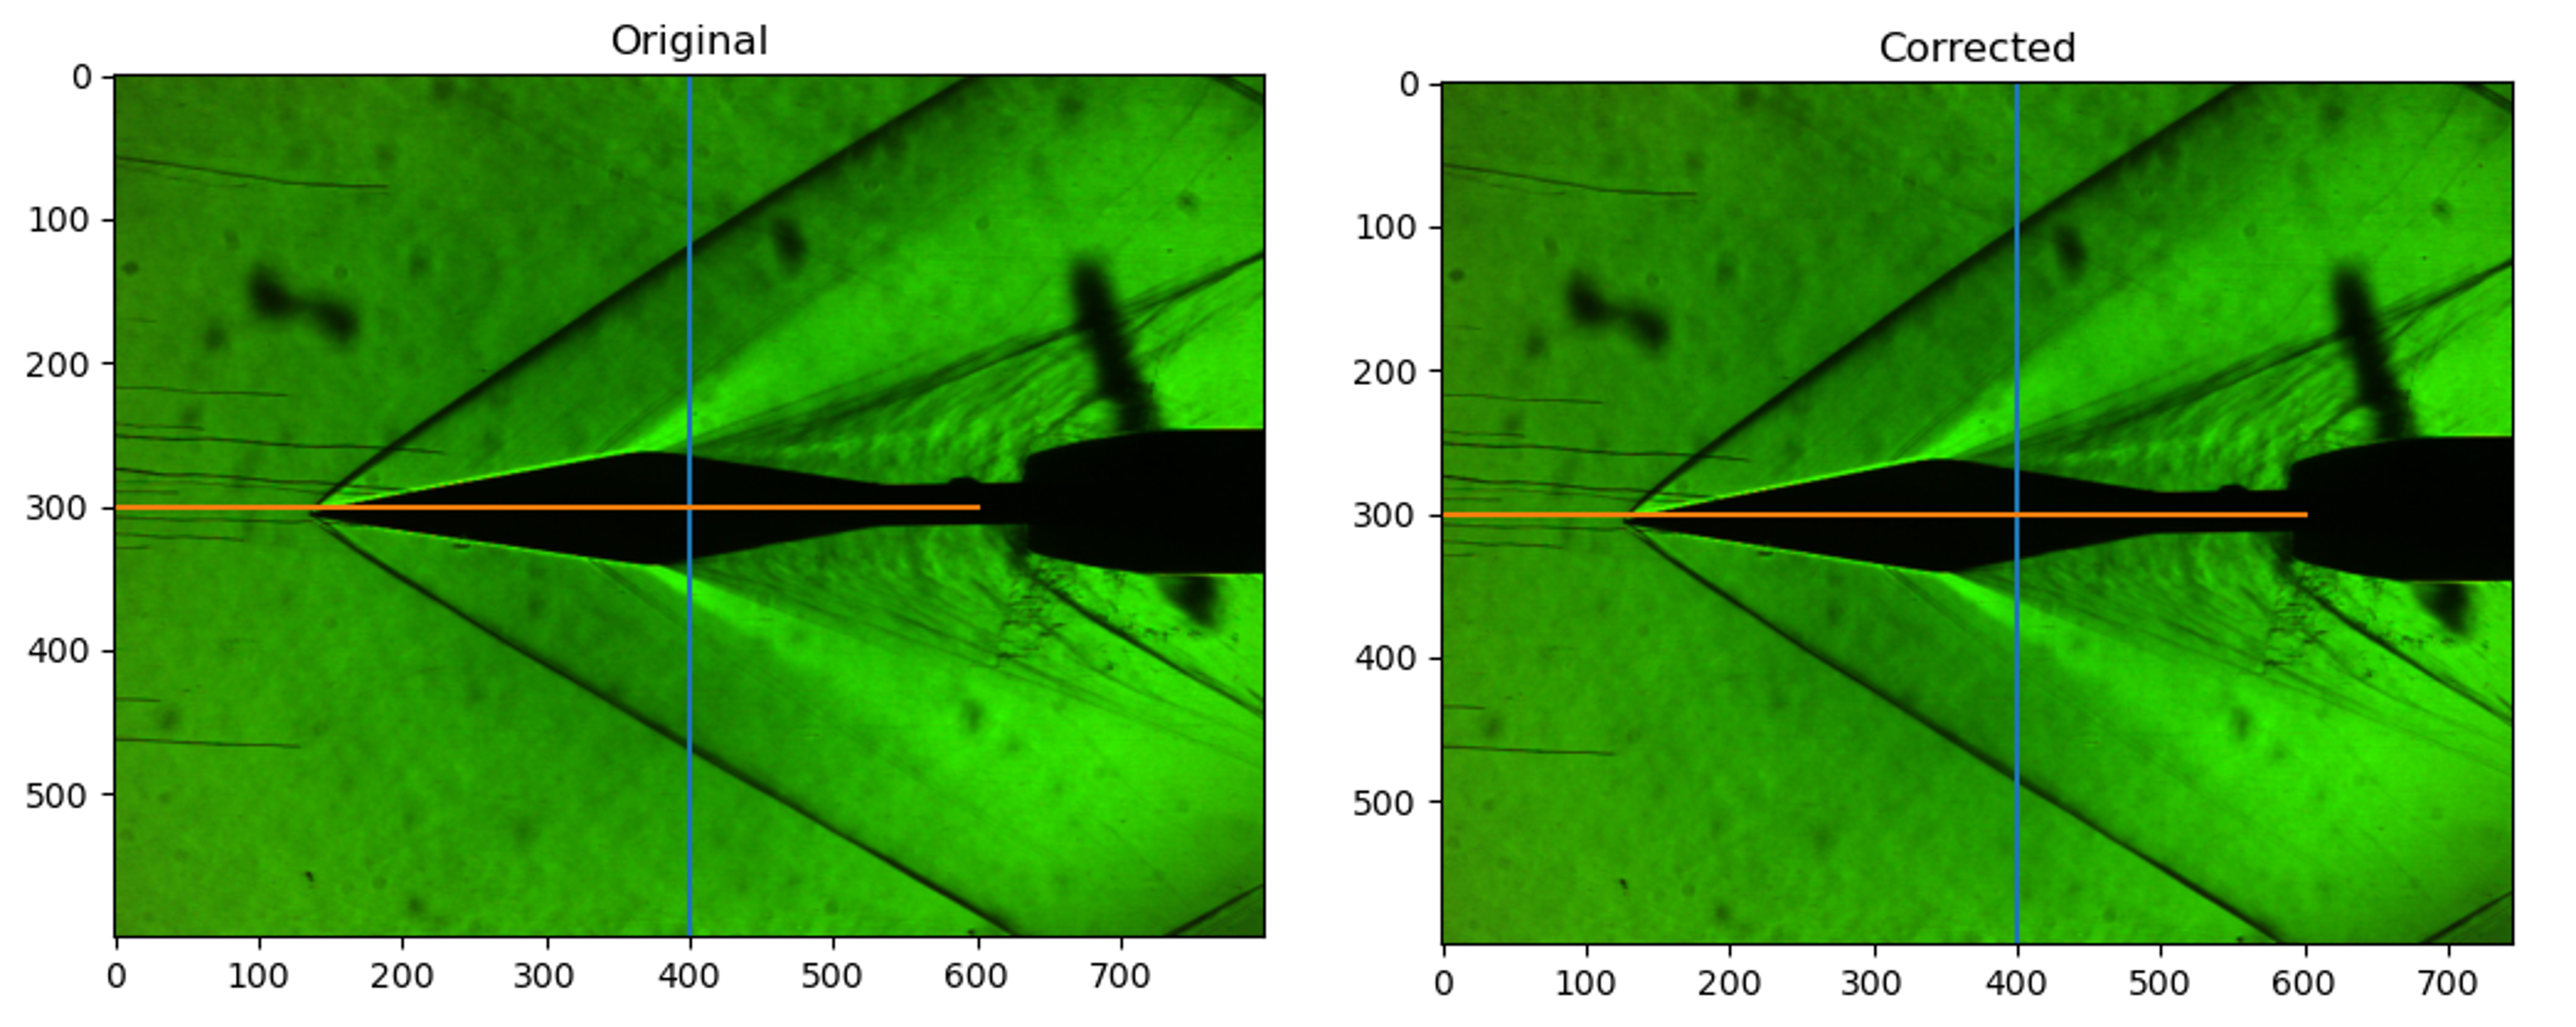
\includegraphics[width = \linewidth]{CorrectedImages/Diamond_AoA0_Mach25_corrected_vs_original.png}
    \caption{Corrected Example with Mach 2.5 flow at $0\degree$ angle of attack, Raw vs Corrected}
    \label{correctionexample}
\end{figure}


\pagebreak


\end{document}